\section{Experiments}

Our experiment settings follow those of the original MeanFlow \cite{mf}, using the same public code.
The experiments are on ImageNet \citep{imagenet} class-conditional generation at 256${\times}$256 resolution. 
Following \cite{shortcut,imm,mf}, the model operates on the latent space of a pretrained VAE tokenizer~\citep{ldm}, which produces 32${\times}$32${\times}$4 latents from 256${\times}$256${\times}$3 images.

We evaluate the challenging protocol of \textbf{1-NFE} generation, where all our models are trained \textbf{\emph{from scratch}}.
We report Fr\'echet Inception Distance (FID)~\citep{fid} on 50K generated images (with additional metrics in \cref{tab:extra-metrics}).
Detailed configurations are in appendix.

\paragraph{Baseline.} 
In our ablations, we use the MeanFlow-B/2 model \cite{mf}.
The ablation models are trained for 240 epochs. Our setting is exactly the same as that of MeanFlow-B/2 in \cite{mf}, which has a 1-NFE FID of 6.17 (with CFG). This model is our starting point.

\begin{figure}[t]
\vspace{-1em}
\centering
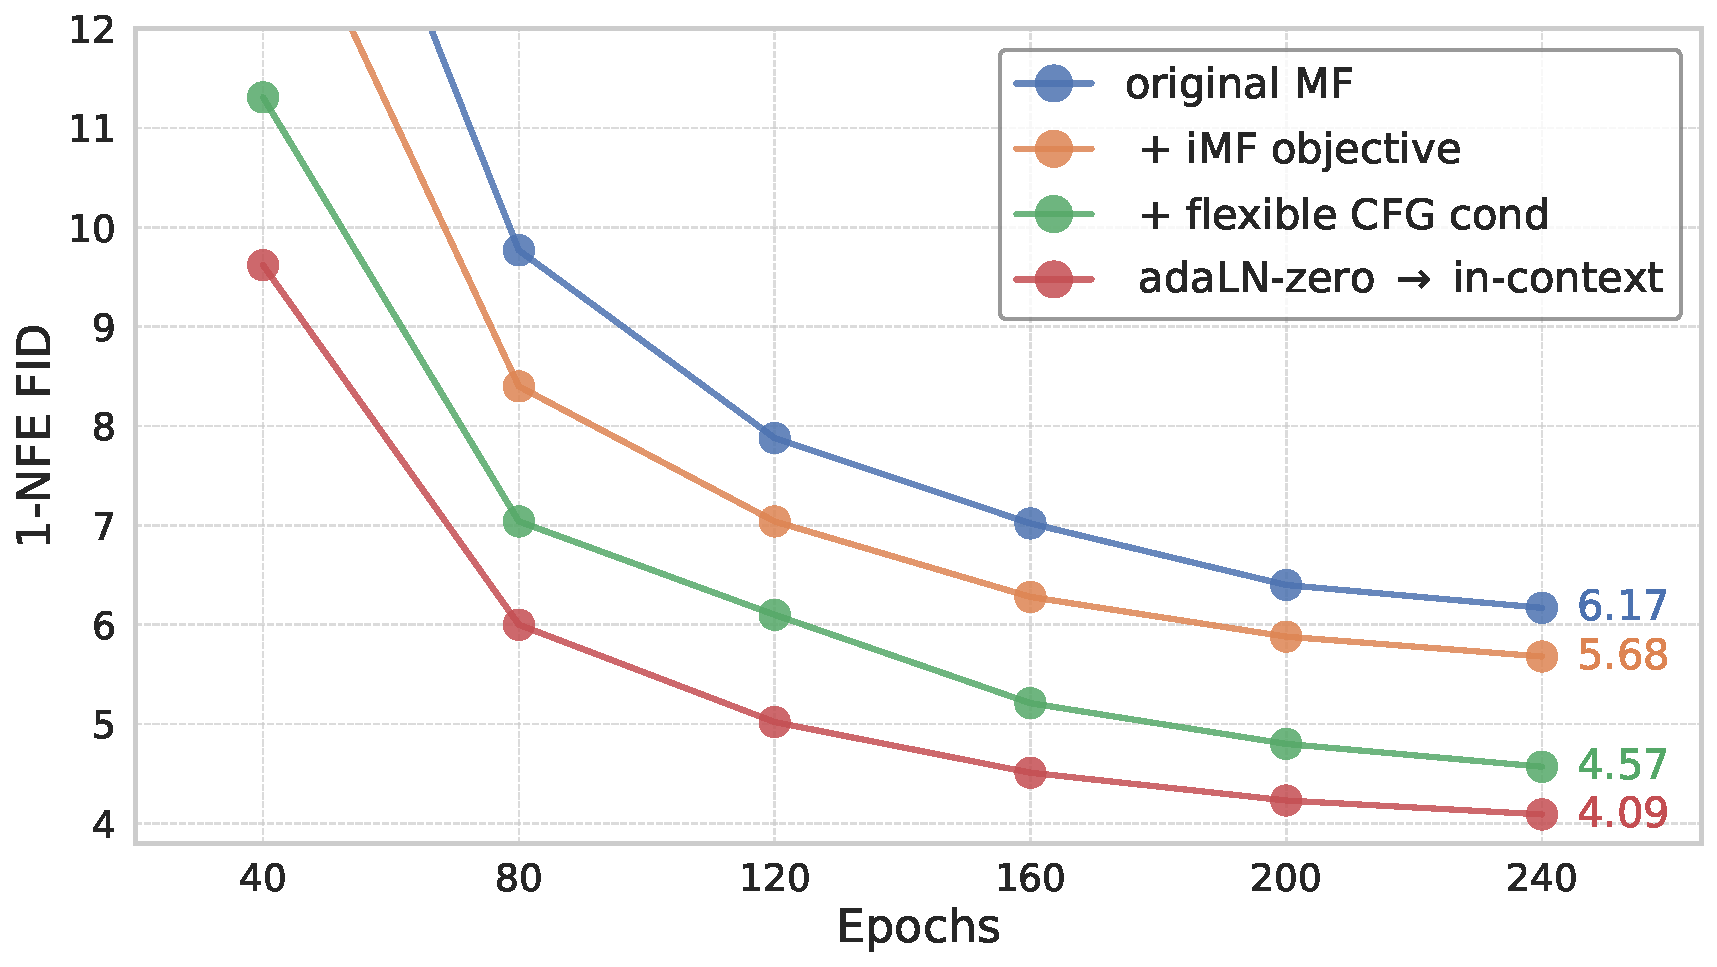
\includegraphics[width=.9\linewidth]{figs/ablation.pdf}
\vspace{-0.7em}
\caption{
\textbf{FID curves during training.} 
The original MeanFlow-B/2 baseline has a 1-NFE FID of 6.17. Using the improved training objective (\cref{sec:v-pred}), FID improves to 5.68. Incorporating flexible CFG conditioning (\cref{sec:method-cfg}) reduces FID to 4.57. Replacing adaLN-zero with in-context conditioning (\cref{sec:method-arch}) further improves FID to 4.09. See also \cref{tab:fid_ablation}.
}
\vspace{-1em}
\label{fig:learning-ablation}
\end{figure}

\subsection{Ablation Study}
\label{sec:ablation}

In \cref{tab:fid_ablation}\textbf{(a)} and \textbf{(b)}, we ablate the iMF designs discussed in \cref{sec:v-pred} and \cref{sec:method-cfg}. The architectural improvements are in \cref{tab:fid_ablation}(c). FID curves during training are in \cref{fig:learning-ablation}.

\paragraph{MeanFlow as $v$-loss.}
In \cref{tab:fid_ablation}\textbf{(a)}, we compare the original MF training formulation (\ref{eq:mf-loss}) with our iMF training formulation (\ref{eq:imf-vpred}). 
We do not use CFG-conditioning here.
We compare two variants of computing $v_\theta$ for the $\mathtt{JVP}$ usage in (\ref{eq:imf-vpred}): the boundary condition or auxiliary head.

When using the variant of boundary condition  ($v_\theta = u_\theta(z_t,t,t)$), our formulation improves the case w/o CFG from an FID of 32.69 to 29.42, representing a solid gain of 3.27. This variant adds no extra parameters at training or inference time. This result demonstrates the impact of the legitimate regression formulation.

When using the auxiliary head variant, our formulation also substantially improves over the original MF, from 32.69 to 30.76 w/o CFG, with a gain of 1.93. While the gain is smaller than that of using the boundary condition, it becomes relatively more significant in the case of ``w/ CFG'', suggesting a more capable model is desired to handle the more challenging scenario.


\begin{table}[t]
\centering
\begin{minipage}{\linewidth}
% ################################################
\begin{subtable}{\linewidth}
\centering
\tablestyle{4pt}{1.1}
\begin{tabular}{y{120}|x{45}|x{45}}
 \textbf{FID, 1-NFE} & w/o CFG & w/ CFG  \\
\hline
original MF~\cite{mf}     & 32.69 & 6.17 \\
our $V_\theta$, with $v_\theta =u_\theta(z_t,t,t)$       & \textbf{29.42} & 5.97 \\
our $V_\theta$, with $v_\theta$ from aux. head         & 30.76 & \textbf{5.68} \\
\end{tabular}
\caption{\textbf{MeanFlow as $v$-loss}. We compare with original MF with our iMF objective in \cref{eq:imf-vpred} in \cref{sec:v-pred}.
We compare two variants of computing $v_\theta$ for \cref{eq:imf-vpred}, namely, using $u_\theta$'s boundary condition or an auxiliary head.
In each row, ``w/o CFG'' and ``w/ CFG'' are two models trained separately, as is in original MF (which does not support flexible inference-time CFG). 
}
\label{subtab:v-pred}
\end{subtable}
\vspace{-0.25em}
\\
\begin{subtable}{\linewidth}
\centering
\tablestyle{4pt}{1.1}
\begin{tabular}{y{120}|x{45}|x{45}}
 \textbf{FID, 1-NFE} & w/o CFG & w/ CFG  \\
\hline
best in \cref{tab:fid_ablation}\textbf{(a)}        &  30.76 & 5.68 \\
% \hline
CFG-condition: $\omega$-condition    &  25.15 & 5.52 \\
CFG-condition: $\Omega$-condition &  \textbf{20.95} & \textbf{4.57} \\
\end{tabular}
\caption{\textbf{Flexible guidance}. Adding guidance as conditioning enables flexible guidance at inference (\cref{sec:method-cfg}).
$\omega$-condition is the basic conditioning on the guidance scale $\omega$.
$\Omega$-condition allows to further condition on CFG interval's start and end points.
Here, only in the first row, ``w/o CFG'' and ``w/ CFG'' are two models trained separately, same as \cref{tab:fid_ablation}\textbf{(a)}; when using our flexible CFG (last two rows), the ``w/o CFG'' cases are simply $\omega=1$ at inference-time, using a single trained model.
}
\label{subtab:flexible-cfg}
\end{subtable}
\vspace{-0.25em}
\\
\begin{subtable}{\linewidth}
\centering
\tablestyle{4pt}{1.1}
\begin{tabular}{y{120}|x{45}|x{45}}
\textbf{FID, 1-NFE} & \# params & w/ CFG \\
\hline
best in \cref{tab:fid_ablation}\textbf{(b)}               & 133M & 4.57             \\
{adaLN-zero $\rightarrow$ in-context cond.} & \textbf{89M} & \textbf{4.09}              \\
\hline
 \deemph{$+$ advanced Transformer blocks} & \deemph{89M} & \deemph{3.82}              \\
\deemph{$+$ longer training (640ep)}  & 
\deemph{89M} & \deemph{3.39} \\
\end{tabular}
\caption{\textbf{In-context conditioning} and other improvements.
Replacing adaLN-zero \cite{dit} with our multi-token in-context conditioning (\cref{sec:method-arch}) improves the results and substantially reduces the model size. Advanced Transformer blocks and longer training yield improvements as expected.}
\label{subtab:arch}
\end{subtable}
% ################################################
% ################################################
% ################################################
\end{minipage}
\vspace{-0.5em}
\caption{\textbf{Ablation study on 1-NFE generation.} FID-50K is evaluated on ImageNet 256$\times$256. All are with the MF-B/2 backbone, trained for 240 epochs from scratch by default.
}
\label{tab:fid_ablation}
\end{table}
%##################################################################################################



In the case of ``w/ CFG'' (here, trained with a fixed $\omega$), using the boundary condition improves FID from 6.17 to 5.97 (\cref{tab:fid_ablation}\textbf{(a)}). While this relative gain is smaller, we observe that the same setting has a more pronounced impact on the same MF-XL model:
\begin{center}
\vspace{-.3em}
\centering\footnotesize
\begin{tabular}{y{120}|c}
\textbf{FID, 1-NFE} & \textbf{MF-XL/2 model}, w/ CFG \\
\hline
original MF~\cite{mf}     
    & 3.43 \\
our $V_\theta$, with $v_\theta = u_\theta(z_t,t,t)$       
    & \textbf{2.99} \\
\end{tabular}
\vspace{-.3em}
\end{center}
We hypothesize that when the model has more capacity, it can better leverage the capacity to learn $v_\theta$ by $u_\theta(z_t,t,t)$, and therefore benefits more from this formulation.

Further, \cref{tab:fid_ablation}\textbf{(a)} shows that the auxiliary head achieves an FID of 5.68 w/ CFG, which is about 10\% relative improvement over the original MF.
This auxiliary head introduces no extra parameters or compute at inference time.
All these comparisons demonstrate that a reliable $v$ estimation \textit{as $\mathtt{JVP}$'s input} is critical for MeanFlow methods.


\paragraph{Flexible guidance.}
In \cref{tab:fid_ablation}\textbf{(b)}, we examine the CFG conditioning proposed in \cref{sec:method-cfg}. This ablation is best examined together with \cref{fig:train-inf-cfg}: the major advantage of CFG conditioning is on the inference-time flexibility, which may not be simply reflected by a single FID number.

In \cref{tab:fid_ablation}\textbf{(b)}, when using the simpler $\omega$-conditioning (\ie only on the CFG scale $\omega$), the FID w/ CFG improves slightly from 5.68 to 5.52. This marginal gain is unsurprising, because the original MF \cite{mf} already had a near-optimal but fixed training-time  $\omega$, for this small model. This gain is more substantial for larger models, for which searching for a fixed training-time $\omega$ becomes impractical.

\cref{tab:fid_ablation}\textbf{(b)} further shows that richer CFG-conditioning (\ie on $\Omega$) substantially improves the FID, by 1.11 to 4.57. This gain is because $\Omega$-conditioning enables CFG interval \cite{interval} \textit{at inference time}, and CFG interval is highly effective even for multi-step methods. 
Our conditioning strategy does not affect the 1-NFE sampling behavior: $(t_\textrm{min}, t_\textrm{max})$ are turned into embeddings for 1-NFE generation.

Interestingly, our CFG conditioning also enables us to mimic the ``w/o CFG'' behavior at inference time. We achieve this by setting $\omega=1.0$ at inference, which represents the ``no CFG'' case (see \cref{eq:cfg}). \cref{tab:fid_ablation}\textbf{(b)} shows that the FID at $\omega=1.0$ (``w/o CFG'') is significantly improved by 10 points, from 30.76 to 20.95. This suggests that training our models across a range of CFG scales can improve their \textit{generalization} performance, substantially improving their results even at a suboptimal $\omega$ value.

\begin{table}[t]
\small
\centering
\tablestyle{4pt}{1.1}
\resizebox{\linewidth}{!}{
\begin{tabular}{y{40}|x{20}x{20}|x{30}x{24}|x{24}x{24}}
{config}       & depth & width & {\# params} & Gflops & {FID}$\downarrow$ & {IS}$\uparrow$ \\
\hline
{MF}-B/2       & 12 & 768  & 131M & 23.1  & 6.17 & 208.0   \\
{MF}-M/2       & 16 & 1024 & 308M & 54.0  & 5.01 & 252.0   \\
{MF}-L/2       & 24 & 1024 & 459M & 80.9  & 3.84 & 250.9   \\
{MF}-XL/2      & 28 & 1152 & 676M & 119.0 & 3.43 & 247.5   \\
\hline
\textbf{iMF}-B/2       & 12 & 768 & 89M  & 24.9  & 3.39 & 255.3    \\
\textbf{iMF}-M/2       & 24 & 768 & 174M & 49.9  & 2.27 & 257.7    \\
\textbf{iMF}-L/2       & 32 & 1024 & 409M & 116.4 & 1.86 & 276.6   \\
\textbf{iMF}-XL/2      & 48 & 1024 & 610M & 174.6 & \textbf{1.72} & \textbf{282.0}   \\
\end{tabular}
}
\vspace{-.75em}
\caption{\textbf{System-level comparison with original MeanFlow}, evaluated by FID and IS \cite{improvedgan} on ImageNet 256$\times$256 with \textbf{1-NFE} generation.
The notations of B/M/L/XL are mainly for reference, as it is impossible to calibrate both model size (\# params) and compute (Gflops) due to the removal of adaLN-zero.
The compute is for 1-NFE of the generator, excluding the tokenizer decoder.
}
\label{tab:extra-metrics}
\vspace{-1.35em}
\end{table}


\begin{table*}[t]
\centering
\vspace{-1.5em}
\resizebox{!}{0.15\linewidth}{
\setlength{\tabcolsep}{4pt}
\small
\begin{tabular}{y{88}x{34}x{24}x{24}}
\toprule
{Method} & {\# Params} & NFE & {FID} \\
\midrule
\rowcolor[gray]{0.9}
\multicolumn{4}{l}{\textit{\textbf{1-NFE diffusion/flow from scratch}}} \\
~~iCT-XL/2~\citep{ict}               & 675M & 1 & 34.24   \\
~~Shortcut-XL/2~\citep{shortcut} & 675M & 1 & 10.60 \\
~~MeanFlow-XL/2~\citep{mf} & 676M & 1 & 3.43   \\
~~TiM-XL/2~\citep{tim} & 664M & 1 & 3.26 \\
~~$\alpha$-Flow-XL/2+~\citep{alphaflow} & 676M & 1 & 2.58 \\
\midrule
~~\textbf{iMF}-B/2 (ours)      & 89M  & 1 & 3.39             \\
~~\textbf{iMF}-M/2 (ours)      & 174M & 1 & 2.27             \\
~~\textbf{iMF}-L/2 (ours)      & 409M & 1 & 1.86             \\
~~\textbf{iMF}-XL/2 (ours)     & 610M & 1 & \textbf{1.72}    \\
\midrule
\rowcolor[gray]{0.9}
\multicolumn{4}{l}{\textit{\textbf{2-NFE diffusion/flow from scratch}}} \\
~~iCT-XL/2~\citep{ict}              & 675M & 2 & 20.30   \\
~~IMM-XL/2~\citep{imm}              & 675M & 1$\times$2 & 7.77 \\
~~MeanFlow-XL/2+~\citep{mf}                  & 676M & 2 & 2.20  \\
~~$\alpha$-Flow-XL/2+~\citep{alphaflow} & 676M & 2 & 1.95\\
\midrule
~~\textbf{iMF}-XL/2 (ours)                       & 610M & 2 & \textbf{1.54}   \\
\bottomrule
\end{tabular}
}
\hspace{.1em}
\resizebox{!}{0.15\linewidth}{
\setlength{\tabcolsep}{4pt}
\textcolor[rgb]{0.6,0.6,0.6}{
% \centering
\small
\begin{tabular}{y{92}x{34}x{30}x{18}}
\toprule
{Method} & {\# Params} & NFE & FID \\
\midrule
\multicolumn{4}{l} {\textit{\textbf{1-NFE diffusion/flow (distillation)}}} \\
~~$\pi$-Flow-XL/2~\citep{piflow} & 675M & 1 & 2.85\\
~~{DMF-XL/2+}~\cite{dmf} & 675M &  1 & 2.16\\
~~FACM-XL/2~\cite{facm} & 675M & 1 & 1.76 \\
\midrule
\multicolumn{4}{l} {\textit{\textbf{Multi-NFE diffusion/flow}}} \\
~~ADM-G~\cite{adm}  & 554M & 250$\times$2 & 4.59 \\
~~LDM-4-G~\cite{ldm}      & 400M & 250$\times$2 & 3.60 \\
~~SimDiff~\cite{simdiff}  & 2B & 1000$\times$2 & 2.77 \\
~~DiT-XL/2~\cite{dit} & 675M & 250$\times$2 & 2.27\\
~~SiT-XL/2~\cite{sit} & 675M   & 250$\times$2 & 2.06  \\
~~SiT-XL/2\;+\;REPA~\cite{repa}      & 675M & 250$\times$2 & 1.42 \\
~~SiD2~\cite{sid2}   & -- & 512$\times$2 & 1.38 \\
~~LightningDiT-XL/2~\cite{vavae} & 675M & 250$\times$2 & 1.35 \\
~~DDT-XL/2~\cite{ddt} & 675M  & 250$\times$2 & 1.26 \\
~~RAE~\cite{rae}\;+\;DiT$^\text{DH}$-XL & 839M & 50$\times$2 & 1.13 \\
\bottomrule
\end{tabular}
}
}
\hspace{.1em}
\resizebox{!}{0.15\linewidth}{
\setlength{\tabcolsep}{4pt}
\textcolor[rgb]{0.6,0.6,0.6}{
\small
\begin{tabular}{y{80}x{34}x{30}x{20}}
\toprule
{Method} & {\# Params} & {NFE} & FID \\
\midrule
\multicolumn{4}{l}{\textit{\textbf{GANs}}} \\
~~BigGAN~\citep{biggan}          & 112M & 1 & 6.95 \\
~~GigaGAN~\citep{gigagan}        & 569M & 1 & 3.45 \\
~~StyleGAN-XL~\citep{styleganxl} & 166M & 1 & 2.30 \\
\midrule
\multicolumn{4}{l}{\textit{\textbf{autoregressive/masking}}} \\
~~JetFormer-L~\cite{jetformer}     & 2.75B & 256$\times$2 & 6.64 \\
~~MaskGIT~\cite{maskgit}               & 227M & 8 & 6.18 \\
~~RQ-Transformer~\cite{RQT}   & 3.8B & 256$\times$2 & 3.80 \\
~~STARFlow~\cite{starflow}                & 1.4B & 1024$\times$2 & 2.40 \\
~~LLamaGen-3B~\cite{llamagen}      & 3.1B & 256$\times$2 & 2.18 \\
~~VAR-$d30$~\cite{var}               & 2B   & 10$\times$2 & 1.92 \\
~~MAR-H~\cite{mar}             & 943M & 256$\times$2 & 1.55 \\
~~RAR-XXL~\cite{rar}               & 1.5B & 256$\times$2 & 1.48\\
~~xAR-H~\cite{xar}                    & 1.1B & 50$\times$2 & 1.24 \\
\bottomrule
\end{tabular}%
}
}
\vspace{-.5em}
\caption{\textbf{System-level comparison on class-conditional ImageNet 256${\times}$256}.
\textbf{Left}: 1-NFE and 2-NFE diffusion/flow models trained \emph{from scratch}.
\textbf{Middle}: Diffusion/flow models, including distillation-based 1-NFE methods and multi-NFE methods.
\textbf{Right}: Reference methods from other generative modeling families, including GANs and autoregressive/masking models.
%
All numbers are with CFG when applicable, and $\times 2$ in NFE indicates that the CFG computation doubles NFEs at inference time.
}
\label{tab:all_results}
\vspace{-.25em}
\end{table*}


\paragraph{In-context conditioning.} 
Thus far, our ablations have been using adaLN-zero \cite{dit} for conditioning. 
In \cref{tab:fid_ablation}\textbf{(c)}, we replace it with our multi-token in-context conditioning (\cref{sec:method-arch}). As adaLN-zero is parameter-heavy, removing it yields a substantial 1/3 reduction in model size, from 133M to 89M. 
Such a reduction is highly attractive for larger models.
The FID is improved from 4.57 to 4.09.

Finally, following \cite{vavae}, we incorporate general-purpose Transformer improvements: SwiGLU \cite{swiglu}, RMSnorm \cite{rmsnorm}, and RoPE \cite{rope}. These components put together improve FID from 4.09 to 3.82.  Training longer yields an extra gain, achieving 3.39 FID with this B-size model.



\subsection{Comparisons with Original MeanFlow} 

In \cref{tab:extra-metrics}, we provide a system-level comparison with the original MF \cite{mf}. We note that removing adaLN-zero makes it impossible to fully calibrate the model sizes, and as such, the B/M/L/XL notations are mainly for the ease of referring. In our designs: \textbf{(i)} the B-size model has the same depth and width in both MF and iMF; \textbf{(ii)} the M-size model is designed to have \textit{smaller} size and \textit{less} compute; and \textbf{(iii)} the L/XL-size models are designed to roughly match the model size of the MF counterparts (yet are still $\app$10\% smaller).

Overall, \cref{tab:extra-metrics} shows that our iMF models have substantially better FID and IS results.
Our iMF-XL/2 model achieves a 1-NFE FID of \textbf{1.72}, representing a \textbf{50\%} relative reduction compared to MF-XL/2’s 3.43. Qualitative examples are in \cref{fig:result_images} and appendix.


%##################################################################################################
\begin{figure}[t]
\centering
\begin{minipage}[t]{\linewidth}
    \centering
    \includegraphics[width=\textwidth]{imgs/12.jpg}
    \\ \vspace{-0.25em}
    {\scriptsize class 12: house finch, linnet, Carpodacus mexicanus}
    \vspace{0.4em}
\end{minipage}

\begin{minipage}[t]{\linewidth}
    \centering
    \includegraphics[width=\textwidth]{imgs/738.jpg}
    \\ \vspace{-0.25em}
    {\scriptsize class 738: pot, flowerpot}
    \vspace{0.4em}
\end{minipage}

\begin{minipage}[t]{\linewidth}
    \centering
    \includegraphics[width=\textwidth]{imgs/975.jpg}
    \\ \vspace{-0.25em}
    {\scriptsize class 975: lakeside, lakeshore}
\end{minipage}

\vspace{-0.5em}
\caption{\textbf{Qualitative results of 1-NFE generation on ImageNet 256$\times$256.}
We show \textit{uncurated} results on the three classes listed here; more are in appendix. The model is iMF-XL/2.
}
\vspace{-0.6em}
\label{fig:result_images}
\end{figure}
%##################################################################################################

\subsection{Comparisons with Previous Methods}  

In \cref{tab:all_results}, we provide system-level comparisons with previous methods. We categorize the methods into:
(i) fastforward generative models trained \textit{from scratch} (\cref{tab:all_results}, left); 
(ii) fastforward generative models, \textit{distilled} from pre-trained multi-step models (\cref{tab:all_results}, mid-top); 
(iii) multi-step diffusion/flow models (\cref{tab:all_results}, mid-bottom); (iv) GAN and autoregressive models (\cref{tab:all_results}, right). 

\paragraph{Fastforward models from scratch.} \cref{tab:all_results} (left) shows that our iMF substantially outperforms other fastforward models that are also trained from scratch. 
In addition, our 1-NFE FID of 1.72 also outperforms those \textit{distilled} from pre-trained models (\cref{tab:all_results}, mid-top), suggesting that training from scratch can produce highly competitive fastforward models.
When relaxing NFE to 2, iMF achieves an FID of \textbf{1.54}. This further closes the gap with the \textit{many-step} diffusion/flow models (\cref{tab:all_results}, mid-bottom).
